\section{Score and Rank}

% intro
\begin{frame}
    \frametitle{Score and Rank: Why?}
    The majority of side-channel attacks employ a \textbf{divide-and-conquer} strategy. \newline
       Instead of targeting the full cipher key at once, the attack partitions it into smaller, more manageable parts. For example, a 16-byte (128-bit) AES key is typically attacked as 16 independent key bytes.
    \vspace{1cm}
    \begin{block}{The Goal}
        This approach allows the attacker to recover each small key part individually, dramatically reducing the complexity of the attack. The metrics of \textbf{score and rank} are used to evaluate the success of recovering each of these parts.
    \end{block}
\end{frame}



% Scorie and Rank Process
\begin{frame}
    \frametitle{The Scoring and Ranking Process}
    \framesubtitle{For a Single Key Part (e.g., one AES key byte)}
    For each key portion:
    \begin{enumerate}
        \item \textbf{Hypothesize:} The attacker considers all possible values for the key part. For an 8-bit key byte, this means 256 key candidates (0 to 255).
        \item \textbf{Score:} A score is computed for each key candidate. This score, generated by a distinguisher like correlation, measures how well the hypothesis for that candidate matches the observed side-channel leakage.
        \item \textbf{Guess:} The scores are sorted to produce an ordered list of guesses, from best to worst. The key candidate with the highest score becomes \texttt{guess\textsubscript{1}}, the attacker's top choice. For instance, if candidate k=42 had the best score, then \texttt{guess\textsubscript{1}} would be 42.
        \item \textbf{Rank:} A rank is assigned to each key candidate based on its position in the sorted list. The best-scoring candidate receives rank 1.
    \end{enumerate}
\end{frame}

\begin{frame}
    \frametitle{Algorithm for a Standard Attack with Score and Rank}
    
    \begin{algorithm}[H]
    \begin{algorithmic}[1] 
        \Statex \textbf{Input:} Attack score function $f(\cdot)$, Key candidates $K$
        \Statex \textbf{Data:} Simulated or real side-channel traces
        \Statex \textbf{Output:} $score_k, guess_k, rank_k$, for all $k \in K$ and all key partitions 
        %\Comment{Partition the full cipher key and attack all key parts}
        \State $partitions \gets \text{divide-and-conquer}(\text{full key})$
        \ForAll{$partition \in partitions$}
            %\Comment{Compute the attack score for every key candidate}
            \ForAll{$k \in K$}
                \State $score_k \gets f(\text{traces}, k)$
            \EndFor
            %\Comment{Sort the scores and compute the key guesses}
            \State $[score_i, score_j, \dots, score_m] \gets \text{sort}([score_0, score_1, \dots, score_{|K|-1}])$
            \State $[guess_1, \dots, guess_{|K|}] \gets [i, j, \dots, m]$
            %\Comment{Compute the rank of every key candidate using the key guesses}
            \ForAll{$guess_i$, with $i \in \{1, 2, \dots, |K|\}$}
                \State $rank_{guess_i} \gets i$
            \EndFor
        \EndFor
    \end{algorithmic}
    \end{algorithm}
\end{frame}

\begin{frame}
    \frametitle{Interpreting the Results: Convergence}
    \begin{itemize}
        \item By plotting score/rank against the number of traces, we can visualize the attack's progress.
        \item \textbf{What to look for:} A key candidate that \textbf{stands out} from the rest.
        \item A successful attack shows \textbf{convergent behavior}: one candidate consistently achieves the highest score (and thus, rank 1) as more traces are added.
        \item \textbf{Example:} Considering a CPA attack on AES-128, key candidate $K=203$ reaches rank 1 after about 15,000 traces and maintains that top position, demonstrating a successful recovery of that key byte (as shown in the following pictures). 
    \end{itemize}
\end{frame}

\begin{frame}
    \frametitle{Example: Score and Rank Plot Convergence}
    \begin{figure}
        \centering
        % Score plot
        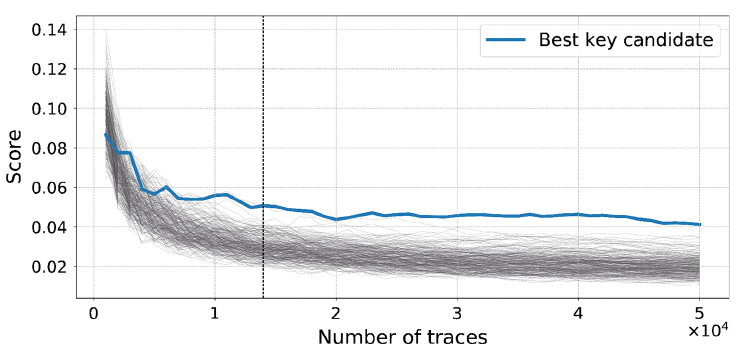
\includegraphics[width=0.55\textwidth]{metrics/Pictures/score_plot.png}
    \end{figure}
    \begin{figure}
        %\vspace{0.5cm} 
        \centering
        % Rank plot 
        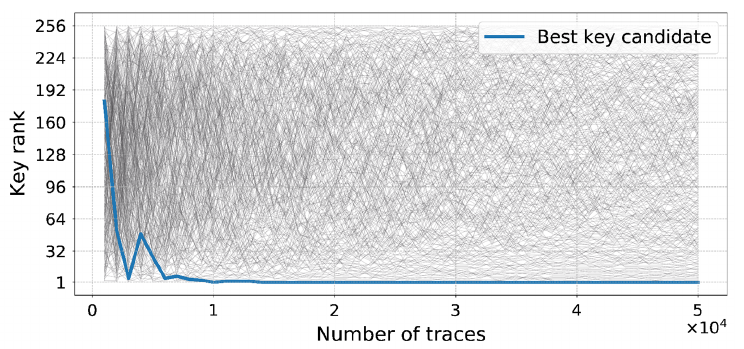
\includegraphics[width=0.55\textwidth]{metrics/Pictures/rank_plot.png}
        \caption{Top: Score plot where the correct key (K=203) is in blue\newline Bottom: Rank plot where the same key's rank converges to 1 after approx. 15,000 traces.}
    \end{figure}
\end{frame}


% Slide 1: Limitation - Statistical Stability
\begin{frame}
    \frametitle{Limitation: Statistical Stability}

    \begin{block}{The pitfall of a single experiment}
        A score/rank plot is typically generated from one traceset and one fixed key. This can be deceptive. \newline
        A single result might be an \textbf{outlier}, as some keys can be accidentally easier or harder to attack than others.
    \end{block}

        To ensure the results are meaningful, we must follow a more rigorous process:
        \begin{itemize}
            \item \textbf{Repeat} the attack multiple times.
            \item \textbf{Vary} the conditions for each run (e.g., use different keys and different sets of traces).
            \item \textbf{Aggregate} the outcomes by calculating the average score/rank and the standard deviation.
        \end{itemize}
        This gives us a \textbf{statistically stable} metric that truly reflects the device's security.
\end{frame}


\begin{frame}
    \frametitle{Limitation: The Full Key Recovery Problem}

        In a real-world attack, the key is unknown. If the attack is suboptimal or uses too few traces, the correct key parts might not achieve Rank 1. Even if the correct byte is at a low rank (like 2 or 3), the \textbf{device is still vulnerable}, but the full key remains hidden.
    
    
    \begin{block}{Key Enumeration}
        To find the full key, the attacker must perform \textbf{key enumeration}. This is a time-consuming, trial-and-error process:
        \begin{itemize}
            \item Construct full key candidates from combinations of the top-ranking key parts.
            \item Test each full key candidate (e.g., by decrypting a known ciphertext) until the correct one is found.
        \end{itemize}
        This is often a computationally expensive task.
    \end{block}
\end{frame}


\begin{frame}
    \frametitle{The Evaluator's Solution: Known-Key Analysis}

    \begin{block}{A More Efficient Approach for Evaluation}
        To assess security without the high cost of key enumeration, evaluators use a different strategy: a \textbf{known-key analysis}.
    \end{block}
    
    \begin{itemize}
        \item In this scenario, the evaluator knows the secret key from the start.
        \item This allows them to check the rank of the \textit{correct key} directly, even if the attack fails to place it at Rank 1.
        \item This answers the question "How close are we to breaking it?" and provides a more precise risk assessment than a simple pass/fail.
    \end{itemize}
    
    \begin{alertblock}{Paving the way for new metrics}
        This concept of known-key analysis is the foundation for the next metrics we will discuss: \textbf{Success Rate (SR)} and \textbf{Guessing Entropy (GE)}.
    \end{alertblock}
\end{frame}


